
\section{État de l'art}

\subsection{Réplication optimiste}

La réplication optimiste~\cite{demers1987epidemic, saito2005optimistic} est un
paradigme de réplication qui consiste à copier la donnée partagée chez chaque
utilisateur. De cette façon, ces derniers peuvent directement modifier les
copies, et ce, même en cas de déconnexions.  Ainsi, les données sont toujours
disponibles et réactives aux changements effectués. Dans un second temps, les
modifications sont disséminées aux autres possesseurs de cette donnée partagée
où elles sont appliquées à la copie locale.

D'après le théorème CAP~\cite{gilbert2002brewer} (\emph{Consistency,
  Availability, Partition tolerence}), il est impossible de passer à l'échelle
tout en garantissant à la fois un fort niveau de cohérence, la disponibilité de
la donnée partagée, et la tolérence aux pannes. La réplication optimiste choisit
de sacrifier le critère de cohérence au profit de la disponibilité et de la
tolérence aux pannes: lorsque tous les changements ont été réçu et appliqués par
tous les participants, les copies doivent converger vers un état identique. Il
s'agit du critère de cohérence correspondant à la cohérence à terme (ou
cohérence inéluctable). Bien qu'il soit possible de garantir d'avantages de
propriétés, notament sur l'ordonnancement des modifications, nous nous
intéresserons principalement à ce critère de cohérence.

\begin{figure}
  \centering
  
\begin{tikzpicture}[scale=1.2]

  \newcommand\X{30pt};
  \newcommand\Y{30pt};
  
  \draw[->](0pt,   0pt)--(10*\X,   0pt);
  \draw[->](0pt, -1*\Y)--(10*\X, -1*\Y);
  \draw[->](0pt, -2*\Y)--(10*\X, -2*\Y);
  
  \draw[fill=black](0pt, 0pt) node[anchor=east]{copie 1 }circle(2pt);
  \draw[fill=black](0pt, -1*\Y) node[anchor=east]{copie 2 }circle(2pt);
  \draw[fill=black](0pt, -2*\Y) node[anchor=east]{copie 3 }circle(2pt);

  \draw(\X,2pt)--node[anchor=south]{[ ]}( \X,   -2pt);
  \draw(\X,2 -1*\Y)--node[anchor=south]{[ ]}(\X,-2 -1*\Y);
  \draw(\X,2 -2*\Y)--node[anchor=south]{[ ]}(\X,-2 -2*\Y);

  \draw(2* \X,2pt)--node[anchor=south]{[QWE]}(2* \X,   -2pt);
%  \draw(2* \X,2 -1*\Y)--node[anchor=south]{[ ]}(2* \X,-2 -1*\Y);
%  \draw(2* \X,2 -2*\Y)--node[anchor=south]{[ ]}(2* \X,-2 -2*\Y);

  \draw[->, dashed] (2*\X, 0pt) -- (8*\X, -1*\Y);
  \draw[->, dashed] (2*\X, 0pt) -- (3*\X, -2*\Y);

  \draw(4*\X, 2 -0*\Y)--node[anchor=south]{[QWE]}(4*\X,-2 -0*\Y);
  \draw(4*\X, 2 -1*\Y)--node[anchor=south]{[ ]}(4*\X,-2 -1*\Y);
  \draw(4*\X, 2 -2*\Y)--node[anchor=south]{[QWE]}(4*\X,-2 -2*\Y);


  \draw(6*\X, 2 -2*\Y)--node[anchor=north]{[QWERTY]}(6*\X,-2 -2*\Y);


  \draw[->, dashed] (6*\X, -2*\Y)--(7*\X, -0*\Y);
  \draw[->, dashed] (6*\X, -2*\Y)--(7*\X, -1*\Y);

  \draw(9*\X, 2 -0*\Y)--node[anchor=south]{[QWERTY]}(9*\X,-2 -0*\Y);
  \draw(9*\X, 2 -1*\Y)--node[anchor=south]{[QWERTY]}(9*\X,-2 -1*\Y);
  \draw(9*\X, 2 -2*\Y)--node[anchor=south]{[QWERTY]}(9*\X,-2 -2*\Y);


%%  \draw[fill=white, very thick]
%%  (0*\X, 0*\Y) node{$p_1$} +(-5pt,-5pt) rectangle +(5pt,5pt);
%%  \draw[->](-5+\X, 5+2*\Y)to[out=120,in=30](0pt,5+2*\Y); %% 6 -> 7
\end{tikzpicture}
  \caption{\label{fig:optimisticexample}Exemple d'execution d'un protocole de
    réplication optimiste. Il existe trois copies d'une séquence initialement
    vide. La première copie insère 'QWE' et en dissémine l'information. La
    troisième copie réçoit l'opération et l'applique localement. Cette copie
    insère 'RTY' à la suite de 'QWE' afin d'obtenir 'QWERTY' et envoie
    l'information aux deux autres copies. Quel que soit l'ordre de reception, le
    protocole garantie que les copies convergent vers un état identique, ici, la
    séquence 'QWERTY'.}
\end{figure}

Les outils d'édition collaboratifs utilisant la réplication optimiste peuvent
être divisés en deux catégories. Les premiers utilisent les transformés
opérationnels~\cite{sun2009contextbased, sun1998operational} qui, lors de la
réception d'une modification, en change les paramêtres égards des opérations
concurrentes. Les seconds utilisent un type de données
commutatif~\cite{shapiro2011comprehensive, shapiro2011conflict} où l'envoie
n'est pas l'opération mais son résultat qui, après reception, est intégré à la
structure. 

\subsection{Transformés opérationnels}

Les approches à transformés opérationnels~\cite{sun2009contextbased,
  sun1998operational} (OT) sont les plus anciennes et s'appliquent à un large
champs d'applications tels que l'édition de texte, l'édition d'images etc. Dans
le cadre de l'édition de texte, OT, en plus des usuels opérations \emph{insert}
et \emph{delete}, apportent des opérations ciblant les chaînes de caractères, à
savoir \emph{move}, \emph{cut -- paste}, etc. Toutefois, l'analyse de correction
nécessite d'examiner chaque paire d'opérations ainsi que leurs paramètres. En
conséquence, lors de l'écriture du papier \cite{imine2003proving}, peu
d'approches étaient réellement correctes. De plus, cette classe d'approches peut
être divisé en deux sous-classes: les approches centralisées et les approches
décentralisées. Les premières réarrangent les opérations sur un serveur
central~\cite{nichols1995high} afin de faciliter la convergence. Toutefois, la
topologie elle-même implique un point individuel de défaillance, des problèmes
de respect de la vie privée, des problèmes d'intelligence économique, des
problèmes de censure, et enfin, de passage à l'échelle. Les approches
décentralisées~\cite{sun2009contextbased}, quant à elle, nécessitent un vecteur
de version afin d'identifier les contextes de génération des opérations
reçues. Elles transforment les arguments de l'opération reçue par rapport aux
opérations concurrentes dans le but d'exécuter de manière cohérente l'opération
sans avoir à défaire et réexecuter ces opérations. De ce fait, bien que
l'exécution locale d'une opération soit très efficace, l'exécution des
opérations reçues est très coûteuse en cas de concurrence. Ainsi, confiné aux
environnements maîtrisés, OT reste efficace (\TODO{REF hybrid paper}).

\subsection{Structures de données partagées pour séquences}

Plus récemment, les approches à base de \emph{structures de données répliqués
  sans résolution de conflits}~\cite{shapiro2011comprehensive,
  shapiro2011conflict} (CRDTs) commencèrent à émerger. Ces types de structure
abstraits possèdent la particularité de fournir des opérations commutatives.
Plus précisément, le résultat de l'éxecution locale de chaque opération est
envoyé aux possésseurs de réplique et peut directement être intégré à cette
dernière.  En d'autres termes, l'ordre d'intégration des opérations n'importe
pas. Cela permet de grandement alléger, voir supprimer, le coût d'ordonnancement
des opérations. Ce genre de structure existe pour les compteurs, les ensembles,
les graphes orientés acycliques (DAG) etc. Dans ce manuscrit, nous nous
interesserons aux séquences.

Une importante différence entre les approches basées sur OT et les approches
basées sur les CRDTs réside dans la répartition des coûts algorithmiques entre
execution locale et intégration distante. En effet, OT propose des opérations
sans coût additionnel localement, mais dont le coût est élevé à l'intégration.
En revanche, les approches CRDTs répartissent les coûts entre la partie locale
et l'intégration.  L'impact étant d'autant plus important qu'une opération local
génére autant d'intégrations que de répliques.

Tandis que les CRDTs améliorent de manière significative la complexité
temporelle des opérations comparé aux approches OT décentralisées, ils
dissimulent leur complexité dans l'occupation mémoire. En effet, afin d'assurer
la convergence des répliques, une opération d'insertion alloue un identifiant
unique  À cet égard, deux types d'approche CRDT existent.

\subsubsection{Pierres tombales}

Les approches utilisant des pierres tombales~\cite{ahmed2011evaluating,
  conway2014language, grishchenko2010deep, oster2006data,
  preguica2009commutative, roh2011replicated, weiss2007wooki, wu2010partial,
  Yu2012stringwise} marquent simplement les éléments supprimés et les cachent à
l'utilisateur. Bien que supprimées, ces pierres tombales existent toujours dans
la structure sous-jacente et continuent d'avoir un impact sur les performances.

Le premier representant historique appartenant à cette famille de CRDT se nomme
WOOT~\cite{oster2006data}. Lors de l'insertion d'un élement dans la sequence,
l'identifiant généré référence simplement les identifiants voisins à
l'insertion. Par exemple, considérons la chaine QWETY dont les identifiants
respectifs à chaque caractère sont $i_Q$,$i_W$,\ldots,$i_Y$. Lors de l'insertion
du caractère R entre les caractères E et T, l'identifiant généré est composé de
$i_E$ et $i_T$ respectivement référencés comme étant la borne inferieur et
supérieur du nouvel élement. Lors de l'intégration, un \TODO{diagramme de Hasse}
permet de retrouver l'ordre des élements de la séquence, même en présence
d'opérations concurrentes. WOOT illustre bien la nécessité de conserver des
pierres tombales après suppression d'un élement. En effet, si l'on supprime un
élement référencé par d'autres élements, alors ces derniers ne peuvent plus être
placé dans le diagramme.

La complexité de ces approches dépend de l'ensemble des opérations d'insertions
ayant jamais été effectué sur le document. Cela devient problématique dans
certains documents particulièrement assujettis à vandalisme (e.g. Wikipedia). La
conséquence étant qu'un document n'ayant en apparence que peu de contenu
consomme beaucoup de ressources du fait des nombreuses pierres tombales cachées.

\TODO{Garbage collect}.

\subsubsection{Identifiants de taille variable}

Les approches utilisant des identifiants de taille
variable~\cite{preguica2009commutative, andre2013supporting,
  weiss2009logoot}. Contrairement aux approches basées sur les pierres tombales,
les éléments supprimés disparaissent complètement de la structure. En
contrepartie, les identifiants encodent un ordre total permettant de les placer
dans le document indépendamment des autres éléments. La complexité spatiale de
ces identifiants est cruciale et dépend du nombre d'opérations d'insertion.

\subsection{Stratégie d'allocation d'identifiants}

Dans la littérature, deux genres de stratégies d'allocations d'identifiants
existent. Tout d'abord, considérons l'insertion de l'élément $b$ entre les
éléments $a$ et $c$ dont les identifiants respectifs sont $id_a$ et $id_c$ avec
$id_a<id_c$. Dans tous les cas, une fonction d'allocation cherche à allouer le
plus petit identifiant possible. Ainsi, l'identifiant généré à une taille
maximum de $min(|id_a|,\, |id_c|)+1$. La première stratégie consiste à allouer
une position aléatoire entre les deux identifiants afin d'éviter au maximum les
conflits dûs à la concurrence. Toutefois, cette stratégie consume en moyenne la
moitié de l'espace entre deux identifiants. La seconde stratégie provient
d'observations faites sur un corpus de textes favorable à l'édition de gauche à
droite. Dans ce genre de cas, la stratégie consiste à rapprocher les
identifiants générés du précédent identifiant (e.g. $id_b$ proche de
$id_a$). Toutefois, lorsque le comportement d'édition ne suit pas celui attendu,
la taille des identifiants croît très rapidement.

\begin{figure*}
  \centering
  \subfloat[Comportement d'édition attendu]
  [\label{fig:compliant}Le comportement d'édition correspond aux attentes
  de la stratégie d'allocation]
  {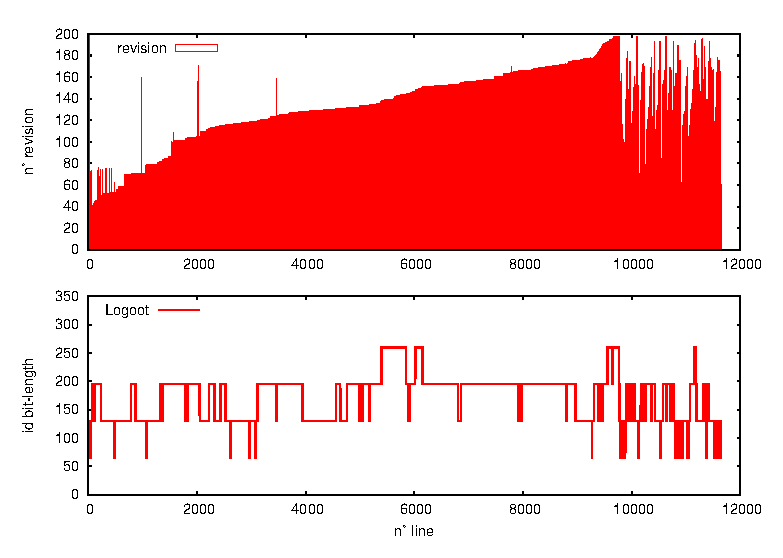
\includegraphics[width=0.48\textwidth]{./img/compliant.eps}}
  \hspace{10pt}
  \subfloat[Comportement d'édition inattendu]
  [\label{fig:motivating}Le comportement d'édition va à l'encontre des attentes
  de la stratégie d'allocation]
  {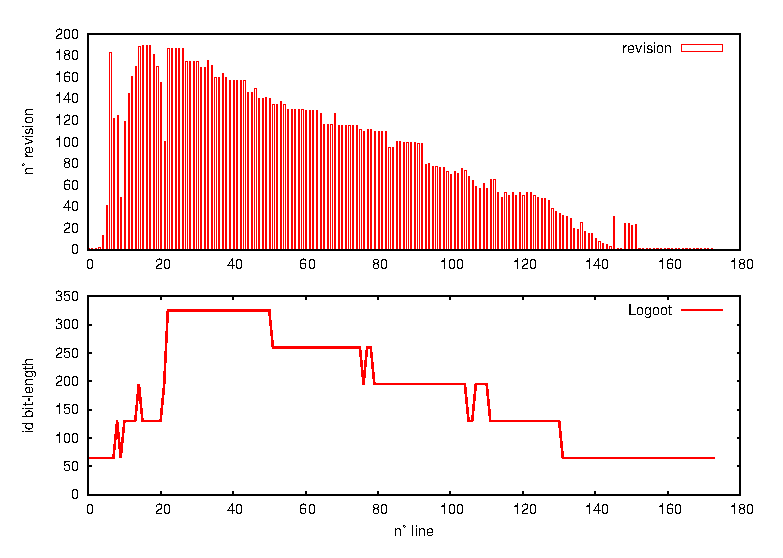
\includegraphics[width=0.48\textwidth]{./img/motivating.eps}}
  \caption{\label{fig:allocation}Spectre de documents Wikipedia sous différent
    comportements d'édition antagonistes. La figure du haut représente la
    révision à laquelle la ligne a été insérée, i.e., sa date de naissance.  La
    figure du bas représente la taille de l'identifiant associé à chaque ligne.}
\end{figure*}

%%% Local Variables:
%%% mode: latex
%%% TeX-master: "../../paper"
%%% End:
